\documentclass[10pt]{beamer}
% \setbeamersize{text margin left=10mm,text margin right=10mm}

% \usepackage[OT1]{fontenc}

\beamertemplatenavigationsymbolsempty

%\usefonttheme{professionalfonts}
%\usepackage{lxfonts}
% \usepackage{mathtools}
% \usepackage{lato}
% \usepackage{unicode-math}
% \setmainfont{Lato}
% \setmathfont{LatoMath.otf}

\usepackage{tikz, tikz-3dplot, tikz-cd, adjustbox, subcaption, changepage}
\usetikzlibrary{knots, hobby, braids}
\usepackage{amsthm}

\usepackage{amsfonts, esint, slantsc, bboldx}
\usepackage{sansmathfonts}

\usetikzlibrary{cd, backgrounds}
\newcommand*\tmnl[2][c]{\begin{tabular}{@{}#1@{}}#2\end{tabular}}

\theoremstyle{definition}
\newtheorem{thm}{Theorem}

\newcommand{\I}{\mathbfbb{I}}

\title{Braids and the Jones polynomial}
\subtitle{Thesis presentation}
\author{Apoorv Potnis}
\institute{IISERB}
\date{April 2023}

\AtBeginSection[]
{
	\begin{frame}
		\frametitle{Table of Contents}
		\tableofcontents[currentsection, currentsubsection]
	\end{frame}
	\frame{\sectionpage}
}
\AtBeginSubsection{\frame{\subsectionpage}}

\newsavebox{\foobox}
\newcommand{\slantbox}[2][0]{\mbox{%
		\sbox{\foobox}{#2}%
		\hskip\wd\foobox
		\pdfsave
		\pdfsetmatrix{1 0 #1 1}%
		\llap{\usebox{\foobox}}%
		\pdfrestore
	}}
\newcommand\unslant[2][-.25]{\slantbox[#1]{$#2$}}
\newcommand{\tauu}{\unslant\tau\!}

\definecolor{beamer@blended}{rgb}{0.2,0.2,0.7}

\begin{document}

	\maketitle

% 	\begin{frame}
% 	    \tableofcontents
% 	\end{frame}

	\section{Outline}

	\begin{frame}[fragile]\vspace{1em}
		\begin{adjustwidth}{-0.5em}{-1.4em}
		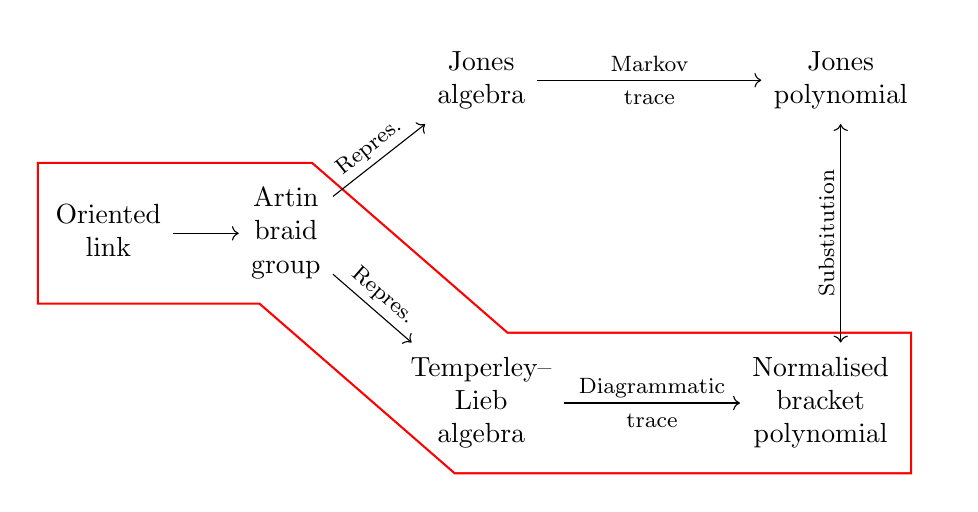
\begin{tikzpicture}[baseline= (a).base]
			\node[scale=1] (a) at (0,0){
				\begin{tikzcd}[
					math mode=false, labels={align=center},
					execute at end picture={
						\scoped[on background layer]
						\draw[red, thick, name prefix=\tikzcdmatrixname-,
						double distance=5em, line cap=rect]
						plot coordinates {(2-1)(2-2)(3-3)(3-4)};}]
					&
					&      \tmnl{Jones \\ algebra}        \arrow[r, "{\footnotesize Markov\\ \footnotesize trace}" auto=false]
					&[4em] \tmnl{Jones \\ polynomial} \\
					\tmnl{Oriented \\ link}        \arrow[r]
					&      \tmnl{Artin \\ braid \\ group} \arrow[rd, sloped, "{\footnotesize Repres.}"]
					\arrow[ru, sloped, "{\footnotesize Repres.}"] \\
					&
					& \tmnl{Temperley-- \\ Lieb \\ algebra}
					\arrow[r, "{\footnotesize Diagrammatic\\ \footnotesize trace}"' auto=false]
					& \tmnl{Normalised\phantom{asd} \\ bracket\phantom{asd} \\ polynomial\phantom{asd}}
					\arrow[uu, leftrightarrow, sloped, "{\footnotesize Substitution}"]
				\end{tikzcd}
			};
		\end{tikzpicture}
		\end{adjustwidth}
	\end{frame}

	\section{Braids}

	\subsection{Geometric definition of braids}

	\begin{frame}
		\frametitle{Three dimensional representation}
		\begin{figure}
		    \centering
			\begin{tikzpicture}
				[scale=1.2,
				cube/.style={thick,black},
				grid/.style={very thin,gray},
				axis/.style={->,beamer@blendedblue,thick}]

				\draw[axis] (0,0,0) -- (6,0,0) node[anchor=west]{$x$};
				\draw[axis] (0,0,0) -- (0,3,0) node[anchor=south]{$y$};
				\draw[axis] (0,0,0) -- (0,0,3) node[anchor=north east]{$z$};

				%draw the top and bottom of the cube
				\draw[cube] (0,0,-1) -- (0,2,-1) -- (5,2,-1) -- (5,0,-1) -- cycle;


				%draw the edges of the cube
				\draw[cube] (0,0,-1) -- (0,0,1);
				\draw[cube] (0,2,-1) -- (0,2,1);
				\draw[cube] (5,0,-1) -- (5,0,1);
				\draw[cube] (5,2,-1) -- (5,2,1);

				\begin{knot}[clip width=8]
					\strand[thick, red] (1,0,0) to [in angle=-90, curve through = {(1,1,0.5)}] (4,2,0) node[black, below]{\(p_1\)};
					\strand[thick, red] (2,0,0) to [in angle=-90, curve through = {(1.7,1.5,0.5)}] (1,2,0) node[black, below]{\(p_2\)};
					\strand[thick, red] (3,0,0) to [in angle=-90, curve through = {(3,0.5,0.7)}] (2,2,0) node[black, below]{\(p_3\)};
					\strand[thick, red] (4,0,0) to [in angle=-90, curve through = {(3,1.3,-0.5)}] (3,2,0) node[black, below]{\(p_4\)};
					\flipcrossings{2}
				\end{knot}

				\node[below, label={\(q_1\)}] at (1,2,0) {};
				\node[below, label={\(q_2\)}] at (2,2,0) {};
				\node[below, label={\(q_3\)}] at (3,2,0) {};
				\node[below, label={\(q_4\)}] at (4,2,0) {};
% 				\node[left, label={O}] at (-0.05,-0.1,0) {};

				\draw[cube] (0,0,+1) -- (0,2,+1) -- (5,2,+1) -- (5,0,+1) -- cycle;

			\end{tikzpicture}
			\caption{Three dimensional geometric representation of a braid}
		\end{figure}
	\end{frame}

	\begin{frame}
		\begin{figure}
			\frametitle{Two dimensional representation}
			\centering
			\begin{tikzpicture}
				[scale=1.5,
				cube/.style={thick,black},
				grid/.style={very thin,gray},
				axis/.style={->,beamer@blendedblue,thick}]

				\draw[axis] (0,0,0) -- (5,0) node[anchor=west]{\(x\)};
				\draw[axis] (0,0,0) -- (0,2.8) node[anchor=south]{\(y\)};

				\begin{knot}[clip width=8]
					\strand[thick, red] (1,0) to [in angle=-90, out angle=90, curve through = {(1.5,1)}] (4,2) node[black, below]{\(p_1\)};
					\strand[thick, red] (2,0) to [in angle=-90, out angle=90, curve through = {(1.7,1.5)}] (1,2) node[black, below]{\(p_2\)};
					\strand[thick, red] (3,0) to [in angle=-90, out angle=90, curve through = {(3,0.5)}] (2,2) node[black, below]{\(p_3\)};
					\strand[thick, red] (4,0) to [in angle=-90, out angle=90, curve through = {(3,1.3)}] (3,2) node[black, below]{\(p_4\)};
					\flipcrossings{2}
				\end{knot}

				\node[below, label={\(q_1\)}] at (1,2) {};
				\node[below, label={\(q_2\)}] at (2,2) {};
				\node[below, label={\(q_3\)}] at (3,2) {};
				\node[below, label={\(q_4\)}] at (4,2) {};
			\end{tikzpicture}
			\caption{A projection of the braid}
			\label{fig:2drepbraids}
		\end{figure}
	\end{frame}

	\begin{frame}
		\frametitle{Multiplication of braids}
		\begin{figure}
			\centering
			\subcaptionbox*{\(b_1\)}{
				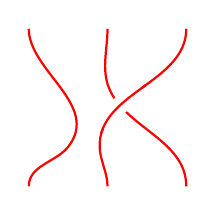
\begin{tikzpicture}[scale=1]
					\begin{knot}[clip width=8]
						\strand[thick, red] (1,0) to [in angle=-90, out angle=90, curve through = {(1.5,0.5)}] (1,2);
						\strand[thick, red] (2,0) to [in angle=-90, out angle=90, curve through = {(1.9,0.5)}] (3,2);
						\strand[thick, red] (3,0) to [in angle=-90, out angle=90, curve through = {(2,1.3)}] (2,2);
					\end{knot}
				\end{tikzpicture}\label{fig:braidmultiplication1}}\qquad\quad
			\subcaptionbox*{\(b_2\)}{
				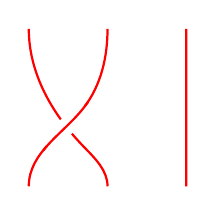
\begin{tikzpicture}[scale=1]
					\begin{knot}[clip width=8]
						\strand[thick, red] (1,0) to [in angle=-90, out angle=90, curve through = {(1.7,1)}] (2,2);
						\strand[thick, red] (2,0) to [in angle=-90, out angle=90, curve through = {(1.7,0.5)}] (1,2);
						\strand[thick, red] (3,0) to [in angle=-90, out angle=90, curve through = {(3,0.5)}] (3,2);
					\end{knot}
				\end{tikzpicture}\label{fig:braidmultiplication2}}\quad\quad\quad
			\subcaptionbox*{\(b_1 b_2\)}{
				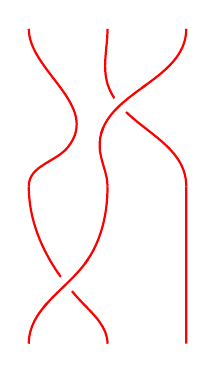
\begin{tikzpicture}[scale=1]
					\begin{knot}[clip width=8]
						\strand[thick, red] (1,0) to [in angle=-90, out angle=90, curve through = {(1.7,1)}] (2,2);
						\strand[thick, red] (2,0) to [in angle=-90, out angle=90, curve through = {(1.7,0.5)}] (1,2);
						\strand[thick, red] (3,0) to [in angle=-90, out angle=90, curve through = {(3,0.5)}] (3,2);
						\strand[thick, red] (1,2) to [in angle=-90, out angle=90, curve through = {(1.5,2.5)}] (1,4);
						\strand[thick, red] (2,2) to [in angle=-90, out angle=90, curve through = {(1.9,2.5)}] (3,4);
						\strand[thick, red] (3,2) to [in angle=-90, out angle=90, curve through = {(2,3.3)}] (2,4);
					\end{knot}
				\end{tikzpicture}\label{fig:braidmultiplication3}}
			\caption{Multiplication of two braids}\label{fig:braidmultiplication}
		\end{figure}
	\end{frame}

	\begin{frame}
		\frametitle{The identity braid \(\I_n\)}
		\begin{figure}\centering
			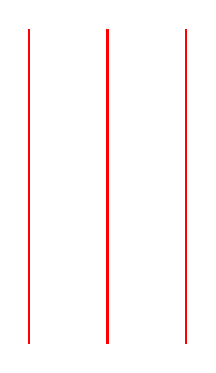
\begin{tikzpicture}[scale=1]
				\begin{knot}[yscale=2, clip width=8]
					\strand[thick, red] (1,0) to (1,2);
					\strand[thick, red] (2,0) to (2,2);
					\strand[thick, red] (3,0) to (3,2);
% 					\flipcrossings{2}
				\end{knot}
			\end{tikzpicture}
			\caption{The identity \(\I_3\)}
			\label{fig:braididentity}
		\end{figure}
	\end{frame}

	\begin{frame}
		\frametitle{Inverse of braids}
		\begin{figure}
			\centering
			\subcaptionbox*{\(b\)}{
				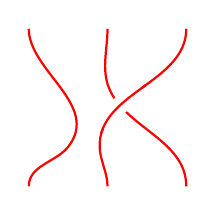
\begin{tikzpicture}[scale=1]
					\begin{knot}[clip width=8]
						\strand[thick, red] (1,0) to [in angle=-90, out angle=90, curve through = {(1.5,0.5)}] (1,2);
						\strand[thick, red] (2,0) to [in angle=-90, out angle=90, curve through = {(1.9,0.5)}] (3,2);
						\strand[thick, red] (3,0) to [in angle=-90, out angle=90, curve through = {(2,1.3)}] (2,2);
						\flipcrossings{2}
					\end{knot}
				\end{tikzpicture}\label{fig:braidinverse1}}\qquad\quad
			\subcaptionbox*{\(b^{-1}\)}{
				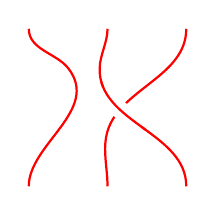
\begin{tikzpicture}[scale=1]
					\begin{knot}[clip width=8, yscale=-1]
						\strand[thick, red] (1,0) to [in angle=-90, out angle=90, curve through = {(1.5,0.5)}] (1,2);
						\strand[thick, red] (2,0) to [in angle=-90, out angle=90, curve through = {(1.9,0.5)}] (3,2);
						\strand[thick, red] (3,0) to [in angle=-90, out angle=90, curve through = {(2,1.3)}] (2,2);
						\flipcrossings{2}
					\end{knot}
				\end{tikzpicture}\label{fig:braidinverse2}}\quad\quad\quad
			\subcaptionbox*{\(b b^{-1} = \I_3\)}{
				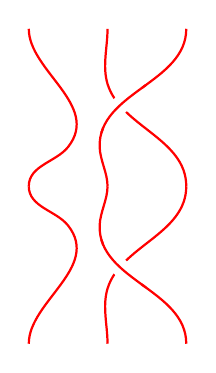
\begin{tikzpicture}[scale=1]
					\begin{knot}[clip width=8]
						\strand[thick, red] (1,0) to [in angle=-90, out angle=90, curve through = {(1.5,0.5)}] (1,2);
						\strand[thick, red] (2,0) to [in angle=-90, out angle=90, curve through = {(1.9,0.5)}] (3,2);
						\strand[thick, red] (3,0) to [in angle=-90, out angle=90, curve through = {(2,1.3)}] (2,2);
						\flipcrossings{2}
						\begin{scope}
							\begin{knot}[clip width=8, yscale=-1]
								\strand[thick, red] (1,0) to [in angle=-90, out angle=90, curve through = {(1.5,0.5)}] (1,2);
								\strand[thick, red] (2,0) to [in angle=-90, out angle=90, curve through = {(1.9,0.5)}] (3,2);
								\strand[thick, red] (3,0) to [in angle=-90, out angle=90, curve through = {(2,1.3)}] (2,2);
								\flipcrossings{2}
							\end{knot}
						\end{scope}
					\end{knot}
				\end{tikzpicture}\label{fig:braidinverse3}}
% 			\quad\quad
% 			\subcaptionbox*{\(\I_3\)}{
% 				\begin{tikzpicture}[scale=0.8]
% 					\begin{knot}[clip width=8, yscale=2]
% 						\strand[thick, red] (1,0) to (1,2);
% 						\strand[thick, red] (2,0) to (2,2);
% 						\strand[thick, red] (3,0) to (3,2);
% 						% \flipcrossings{2}
% 					\end{knot}
%
% 					%\node[below, label={\(q_1''\)}] at (1,4) {};
% 					%\node[below, label={\(q_2''\)}] at (2,4) {};
% 					%\node[below, label={\(q_3''\)}] at (3,4) {};
%
% 					%\node at (2, -1.2) {\(b_1 b_2\)};
% 				\end{tikzpicture}\label{fig:braidinverse4}}
			\caption{Inverse of a braid}\label{fig:braidinverse}
		\end{figure}
	\end{frame}

	\begin{frame}
	    Thus, braids form a group, known as the Artin braid group.
	\end{frame}

	\subsection{Generators and relations}

	\begin{frame}\vspace{1em}
		\frametitle{Generators of the braid group}
		\begin{figure}
			\centering
			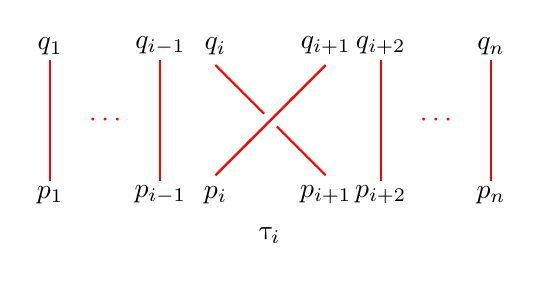
\begin{tikzpicture}[scale=0.7]
				\begin{knot}[clip width=8]
					\strand[thick, red] (-3,-0.1) to (-3,2.1);
					\strand[thick, red] (-1,-0.1) to (-1,2.1);
					\strand[thick, red] (0,0) to (2,2);
					\strand[thick, red] (2,0) to (0,2);
					\strand[thick, red] (3,-0.1) to (3,2.1);
					\strand[thick, red] (5,-0.1) to (5,2.1);
				\end{knot}
				\node[ultra thick, red] at (-2,1) {\(\cdots\)};
				\node[ultra thick, red] at (4,1) {\(\cdots\)};

				\node[below, label={\(p_1\)}] at (-3,-0.7) {};
				\node[below, label={\(p_{i-1}\)}] at (-1,-0.7) {};
				\node[below, label={\(q_1\)}] at (-3,2) {};
				\node[below, label={\(q_{i-1}\)}] at (-1,2) {};
				\node[below, label={\(q_i\)}] at (0,2) {};
				\node[below, label={\(q_{i+1}\)}] at (2,2) {};
				\node[below, label={\(p_i\)}] at (0,-0.7) {};
				\node[below, label={\(p_{i+1}\)}] at (2,-0.7) {};
				\node[below, label={\(p_{i+2}\)}] at (3,-0.7) {};
				\node[below, label={\(p_{n}\)}] at (5,-0.7) {};
				\node[below, label={\(q_{i+2}\)}] at (3,2) {};
				\node[below, label={\(q_{n}\)}] at (5,2) {};

				\node at (1, -1.1) {\(\tauu_i\)};

				\end{tikzpicture}

				\vspace{12pt}

				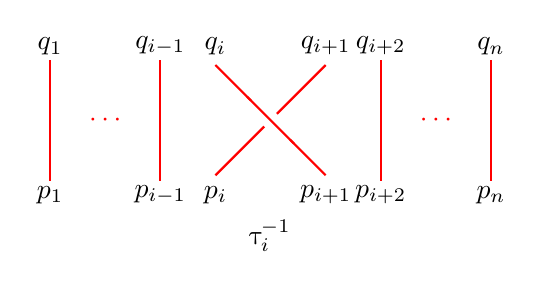
\begin{tikzpicture}[scale=0.7]
					\begin{knot}[clip width=8]
						\strand[thick, red] (-3,-0.1) to (-3,2.1);
						\strand[thick, red] (-1,-0.1) to (-1,2.1);
						\strand[thick, red] (0,0) to (2,2);
						\strand[thick, red] (2,0) to (0,2);
						\strand[thick, red] (3,-0.1) to (3,2.1);
						\strand[thick, red] (5,-0.1) to (5,2.1);
						\flipcrossings{1}
					\end{knot}
					\node[ultra thick, red] at (-2,1) {\(\cdots\)};
					\node[ultra thick, red] at (4,1) {\(\cdots\)};

					\node[below, label={\(p_1\)}] at (-3,-0.7) {};
					\node[below, label={\(p_{i-1}\)}] at (-1,-0.7) {};
					\node[below, label={\(q_1\)}] at (-3,2) {};
					\node[below, label={\(q_{i-1}\)}] at (-1,2) {};
					\node[below, label={\(q_i\)}] at (0,2) {};
					\node[below, label={\(q_{i+1}\)}] at (2,2) {};
					\node[below, label={\(p_i\)}] at (0,-0.7) {};
					\node[below, label={\(p_{i+1}\)}] at (2,-0.7) {};
					\node[below, label={\(p_{i+2}\)}] at (3,-0.7) {};
					\node[below, label={\(p_{n}\)}] at (5,-0.7) {};
					\node[below, label={\(q_{i+2}\)}] at (3,2) {};
					\node[below, label={\(q_{n}\)}] at (5,2) {};

					\node at (1, -1.1) {\(\tauu_i^{-1}\)};
				\end{tikzpicture}

			\caption{Generators \(\tauu_i\) and \(\tauu_i^{-1}\)}
			\label{fig:geometricbraidgenerators}
		\end{figure}
	\end{frame}

	\begin{frame}
		\frametitle{Type II move: \(\tauu_i \tauu_i^{-1} = \I_n\)}
		\begin{figure}
			\centering
			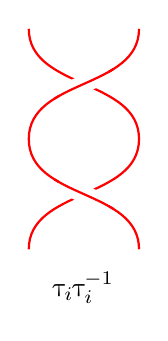
\begin{tikzpicture}
				[scale=0.7]

				\begin{knot}[clip width=8]
					\strand[thick, red] (0,0) to [in angle=-90, out angle=90, curve through = {(2,2)}] (0,4);
					\strand[thick, red] (2,0) to [in angle=-90, out angle=90, curve through = {(0,2)}] (2,4);
					\flipcrossings{1,2}
				\end{knot}

				\node at (1, -0.7) {\(\tauu_i \tauu_i^{-1}\)};
			\end{tikzpicture}
			\quad\quad\quad\quad
			\begin{tikzpicture}
				[scale=0.7]

				\begin{knot}[clip width=8]
					\strand[thick, red] (0,0) to (0,4);
					\strand[thick, red] (2,0) to (2,4);
					\flipcrossings{1,2}
				\end{knot}

				\node at (1, -0.7) {\(\I_n\)};
			\end{tikzpicture}

			\captionof{figure}{A type II move illustrating \(\tauu_i \tauu_i^{-1} = \I_n\)}
			\label{fig:type2}
		\end{figure}
	\end{frame}


	\begin{frame}
		\frametitle{Type III move: \(\tauu_i\, \tauu_{i+1} \tauu_i = \tauu_{i+1} \tauu_i\, \tauu_{i+1}\)}
		\begin{figure}\centering
			\begin{tikzpicture}
				[scale=0.6]

				\begin{knot}[clip width=6]
					\strand[ultra thick, beamer@blendedblue] (0,0) to [in angle=-90, out angle=90, curve through = {(2,2) (4,4)}] (4,6);
					\strand[thick, red] (2,0) to [in angle=-90, out angle=90, curve through = {(0,2) (0,4)}] (2,6);
					\strand[thick, red] (4,0) to [in angle=-90, out angle=90, curve through = {(4,2) (2,4)}] (0,6);
				\end{knot}

				\node at (2, -0.7) {\(\tauu_i\, \tauu_{i+1} \tauu_i\)};
			\end{tikzpicture}
			\quad\quad\quad\quad
			\begin{tikzpicture}
				[scale=0.6]

				\begin{knot}[clip width=6]
					\strand[ultra thick, beamer@blendedblue] (0,0) to [in angle=-90, out angle=90, curve through = {(0,2) (2,4)}] (4,6);
					\strand[thick, red] (2,0) to [in angle=-90, out angle=90, curve through = {(4,2) (2,4)}] (2,6);
					\strand[thick, red] (4,0) to [in angle=-90, out angle=90, curve through = {(2,2) (0,4)}] (0,6);
					%\flipcrossings{1,2}
				\end{knot}

				\node at (2, -0.7) {\(\tauu_{i+1} \tauu_i\, \tauu_{i+1}\)};
			\end{tikzpicture}

			\captionof{figure}{A type III move illustrating \(\tauu_i\, \tauu_{i+1} \tauu_i = \tauu_{i+1} \tauu_i\, \tauu_{i+1}\)}
			\label{fig:type3}
		\end{figure}
	\end{frame}

	\begin{frame}
		\frametitle{Sliding of crossings: \(\tauu_i\, \tauu_j = \tauu_j\, \tauu_i\)}
		\begin{figure}\centering
			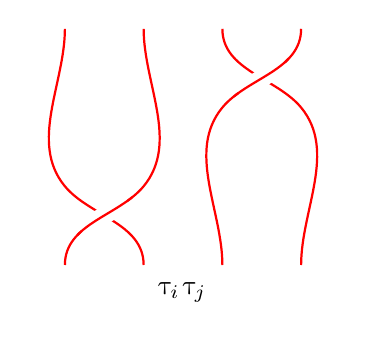
\begin{tikzpicture}
				[scale=0.5]

				\begin{knot}[clip width=8]
					\strand[thick, red] (0,0) to [in angle=-90, out angle=90, curve through = {(2,2)}] (2,6);
					\strand[thick, red] (2,0) to [in angle=-90, out angle=90, curve through = {(0,2)}] (0,6);
					\strand[thick, red] (4,0) to [in angle=-90, out angle=90, curve through = {(4,4)}] (6,6);
					\strand[thick, red] (6,0) to [in angle=-90, out angle=90, curve through = {(6,4)}] (4,6);
				\end{knot}

				\node at (3, -0.7) {\(\tauu_i\, \tauu_j\)};
			\end{tikzpicture}
			\quad\quad\quad\quad
			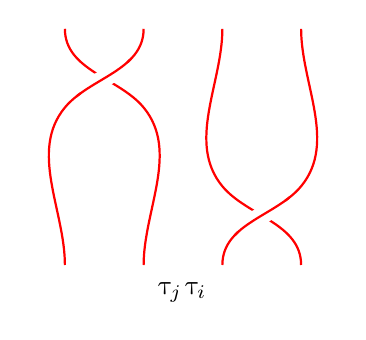
\begin{tikzpicture}
				[scale=0.5]

				\begin{knot}[clip width=8]
					\strand[thick, red] (0,0) to [in angle=-90, out angle=90, curve through = {(0,4)}] (2,6);
					\strand[thick, red] (2,0) to [in angle=-90, out angle=90, curve through = {(2,4)}] (0,6);
					\strand[thick, red] (4,0) to [in angle=-90, out angle=90, curve through = {(6,2)}] (6,6);
					\strand[thick, red] (6,0) to [in angle=-90, out angle=90, curve through = {(4,2)}] (4,6);
					%\flipcrossings{1,2}
				\end{knot}

				\node at (3, -0.7) {\(\tauu_j\, \tauu_i\)};
			\end{tikzpicture}

			\captionof{figure}{Sliding of crossings illustrating \(\tauu_i\, \tauu_j = \tauu_j\, \tauu_i\)}
			\label{fig:sliding}
		\end{figure}
	\end{frame}


\end{document}
